\chapter{Verificación simbólica de modelos}

El algoritmo de verificación de modelos con estados explícitos para Cálculo-$\mu$ presentado anteriormente tiene un problema, es muy susceptible a que ocurra una explosión en el tamaño del modelo, especialmente si el grafo de transición de estados se extrae de un sistema concurrente con muchos componentes. En esta sección se describe un algoritmo de verificación de modelos simbólicos para Cálculo-$\mu$ que opera sobre estructuras de Kripke, esta vez representadas no de manera explícita, sino de manera simbólica a través de fórmulas lógicas.

\section{Representación de fórmulas lógicas}

Los árboles binarios de decisión ordenados (OBDDs) son formas canónicas de representación de fórmulas lógicas. Son considerablemente mas compactos que las formas normales tradicionales como la forma normal conjuntiva y la forma normal disyuntiva, y pueden ser manipulados eficientemente. Por esto, los OBDDs han sido utilizados ampliamente para una variedad de aplicaciones en el diseño asistido por computadoras, incluyendo simulacion simbólica, verificación de lógica combinatoria y, mas recientemente, verificación de sistemas concurrentes con estados finitos.

Para entender la necesidad de usar OBDDs, consideremos primero los árboles binarios de decisión. Un arbol binario de decisión es un árbol dirigido con raiz que consiste en vertices terminales y no terminales. Cada vertice no terminal $v$ esta etiquetado por una variable $var(v)$ y tiene dos hijos: $izq(v)$ corresponde al caso en que $v$ tenga el valor 0 y $der(v)$ en caso contrario. Cada vértice terminal esta etiquetado por una constante $valor(v)$ la cual es 0 o 1. Un árbol binario de decisión para la fórmula $f(a,b,c) = (a \land b) \lor (a \land c)$ es mostrado en la figura \label{fig:kripke1}. Uno puede decidir si una asignación particular a las variables hace verdadera la fórmula o no al atravesar el árbol desde la raíz hasta un vertice terminal. Por ejemplo, la asignación $\{ a \gets 1, b \gets 0, c \gets 0\}$ lleva al vértice terminal 0, por lo tanto la fórmula es falsa para esta asignación.

\begin{figure}[h]
  \centering
  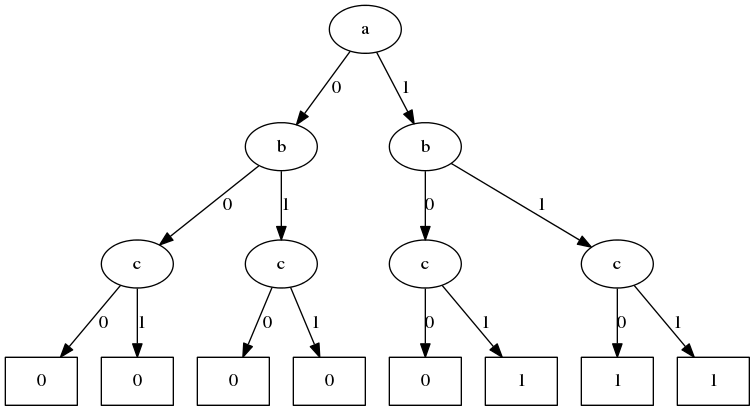
\includegraphics[width=1\textwidth]{Figures/BDT.png}
  \caption{Árbol binario de decisión para este ejemplo.}
  \label{fig:bdt1}
\end{figure}

Los árboles binarios de decisión no proveen una representación muy concisa para las funciones lógicas. De hecho, tienen el mismo tamaño que las tablas de verdad. Afortunadamente, es común que haya mucha redundancia en tales árboles. Por ejemplo, en la figura \label{fig:bdt1} todos los caminos donde a tiene el valor 0 llevan al nodo terminal 0, por lo tanto no seria necesario analizar los valores de $b$ y $c$ en esta rama. Esto lleva a pensar que hay formas de reducir el tamaño del árbol unificando subárboles isomorfos. Esto da como resultado un grafo acíclico dirigido (DAG) llamado diagrama binario de decisión (BDD). Mas precisamente, un BDD es un grafo con raiz, dirigido y acíclico con dos tipos de vertices, vertices terminales y no terminales. Estos tienen el mismo significado que en el caso de los árboles. Cada BDD $B$ con raiz $v$ determina una función lógica $f_{v}(x_{1},...,x_{n})$ de la siguiente manera:

1. Si $v$ es un vértice terminal:
  (a) Si $valor(v) = 1$ entonces $f_{v}(x_{1},...,x_{n}) = 1$.
  (b) Si $valor(v) = 0$ entonces $f_{v}(x_{1},...,x_{n}) = 0$.

2. Si $v$ es un vértice no terminal con $var(v) = x_{i}$ entonces $f_{v}$ es la función 
\[f_{v}(x_{1},...,x_{n}) = (\neg x_{i} \land f_{izq(v)}(x_{1},...,x_{n})) \lor (x_{i} \land f_{der(v)}(x_{1},...,x_{n}))\]



\section{Diagramas binarios de decisión}



